% Appendix A
\chapter{Simulation Settings} % Main appendix title
\label{SimulationSettings} % For referencing this appendix elsewhere, use \ref{AppendixA}

\lhead{Appendix A. \emph{Simulation Settings}} % This is for the header on each page - perhaps a shortened title


\section{Environment}
Settings used in the VoxCad simulation environment are given in table~\ref{VoxelyzeSimulationSettings}.

\begin{table}[ht!]
\centering
\caption{Voxelyze simulation settings}
\label{VoxelyzeSimulationSettings}
    \begin{tabular}{l r p{9cm}}
    \toprule
    \textbf{Property} & \textbf{Value} & \textbf{Description}\\
    \midrule
    \emph{DtFrac} & 0.9 & The timestep of the simulation, currently $0.9 \times dt$, where $dt$ is the optimal timestep.\\
    \emph{ColSystem}        & 3 & Hierarchical collision detection between all voxels. Updates potential collision list only when aggregated motion requires it\footnote.\\
    \emph{StopConditionValue} & 0.4 & Time in seconds simulation is stopped.\\
    \emph{TempBase} & 25.0 & Base temperature of the environment.\\
    \emph{TempAmp} & 39.0 & Temperature's amplitude of the environment.\\
    \emph{TempPeriod} & 0.025 & Period of the temperature cycle.\\
    \emph{Lattice\_Dim} & 0.001 & Lattice dimensions, each voxel has length, height, and depth of $1$mm.\\
    \bottomrule
    \end{tabular}
\end{table}

\footnotetext{From VoxCad's documentation~\cite{hiller2012dynamic}.}



\section{Materials}

\begin{table}[ht!]
\centering
\caption{Universal material properties}
\label{UniversalMaterialProperties}
    \begin{tabular}{l r p{7cm}}
    \toprule
    \textbf{Property} & \textbf{Value} & \textbf{Description}\\
    \midrule
    Poisson's ratio & 0.35 &  It is the ratio of expansion over two other axes following the compression in one.\\
    Density & $1\times10^{6}\   Kg/m^3$ & Density of material.\\
    Temp phase & 0 & Phase of material to temperature period.\\
    Static friction coef. & 1 & Static friction coefficient.\\
    Dynamic friction coef. & 0.5 & Dynamic friction coefficient.\\
    \bottomrule
    \end{tabular}
\end{table}

In this section all materials' properties used during the simulations will be given. All materials used in the simulations have a set of shared properties which are shown in table~\ref{UniversalMaterialProperties}. Furthermore, unique characteristics of the materials are presented in table~\ref{UniqueMaterialProperties}.

\begin{table}[ht!]
\centering
\caption{Unique per material properties}
\label{UniqueMaterialProperties}
    \begin{tabular}{llrr}
    \toprule
    \textbf{Name}                & \textbf{Color} & \textbf{Elastic Modulus} (MPa) & \textbf{CTE} ($1/deg\ C$) \\
    \midrule
    \emph{Active positive} (+) & Red   & 10                    & +0.01\\
    \emph{Active negative} (-) & Green & 10                   & -0.01 \\
    \emph{Passive soft}       & Cyan  & 10                   & 0.00 \\
    \emph{Passive hard}        & Blue  & 50                   & 0.00\\
    \bottomrule
    \end{tabular}
\end{table}















\chapter{Experimental Settings} % Main appendix title
\label{ExperimentalSettings} % For referencing this appendix elsewhere, use \ref{AppendixA}

\lhead{Appendix B. \emph{Experimental Settings}} % This is for the header on each page - perhaps a shortened title

In this section the settings used for each experiment will be presented. For all the following experimental constants the simulation and material settings used are the ones described above, in case of other settings used, the new settings will be mentioned.
\section{Lattice dimension $5^3$}
\label{Settings-size5}
\begin{small}
\begin{description}
\item[Objective function]{Displacement in body lengths (displacement divided by size of soft robot) of soft robot's center of mass.}
\item[Gravity acceleration]{$-27.6\ m/s^2$}
\item[Lattice dimensions]{$5 \times 5 \times 5$}
\end{description}
\end{small}

\section{Lattice dimension $7^3$}
\label{Settings-size7}
\begin{small}
\begin{description}
\item[Objective function]{Displacement in body lengths (displacement divided by size of soft robot) of soft robot's center of mass.}
\item[Gravity acceleration]{$-27.6\ m/s^2$}
\item[Lattice dimensions]{$7 \times 7 \times 7$}
\end{description}
\end{small}

\section{Lattice dimension $10^3$}
\label{Settings-size10}
\begin{small}
\begin{description}
\item[Objective function]{Displacement in body lengths (displacement divided by size of soft robot) of soft robot's center of mass.}
\item[Gravity acceleration]{$-27.6\ m/s^2$}
\item[Lattice dimensions]{$10 \times 10 \times 10$}
\end{description}
\end{small}

\section{Lattice dimension $10^3$-Lunar}
\label{Settings-size10-moon}
\begin{small}
\begin{description}
\item[Objective function]{Displacement in body lengths (displacement divided by size of soft robot) of soft robot's center of mass.}
\item[Gravity acceleration]{$-1.622\ m/s^2$}
\item[Lattice dimensions]{$10 \times 10 \times 10$}
\end{description}
\end{small}

\section{Lattice dimension $10^3$-Mars}
\label{Settings-size10-mars}
\begin{small}
\begin{description}
\item[Objective function]{Displacement in body lengths (displacement divided by size of soft robot) of soft robot's center of mass.}
\item[Gravity acceleration]{$-3.711\ m/s^2$}
\item[Lattice dimensions]{$10 \times 10 \times 10$}
\end{description}
\end{small}

\section{Lattice dimension $10^3$-Earth}
\label{Settings-size10-earth}
\begin{small}
\begin{description}
\item[Objective function]{Displacement in body lengths (displacement divided by size of soft robot) of soft robot's center of mass.}
\item[Gravity acceleration]{$-9.780\ m/s^2$}
\item[Lattice dimensions]{$10 \times 10 \times 10$}
\end{description}
\end{small}

\section{Lattice dimension $10^3$-Jupiter}
\label{Settings-size10-jupiter}
\begin{small}
\begin{description}
\item[Objective function]{Displacement in body lengths (displacement divided by size of soft robot) of soft robot's center of mass.}
\item[Gravity acceleration]{$-24.790\ m/s^2$}
\item[Lattice dimensions]{$10 \times 10 \times 10$}
\end{description}
\end{small}

\section{Gravity Experiments}
\label{gravitySettings}
\begin{small}
\begin{description}
\item[Objective function]{Displacement in body lengths (displacement divided by size of soft robot) of soft robot's center of mass.}
\end{description}
\end{small}
\begin{table}[ht!]
\centering
\caption{Unique per material properties}
\label{UniqueGravitySettings}
    \begin{tabular}{lrrrr}
    \toprule
    \textbf{Planet} & \textbf{Dim.} & \textbf{Grav.} ($m/s^2$) & \textbf{Sim. Time} (Secs.) & \textbf{Temp. Period} (secs.) \\
    \midrule
    Lunar & $7^3$ & -1.622 & 1.0 & 0.050 \\
    Mars & $7^3$ & -3.711 & 1.0 & 0.050 \\
    Earth & $7^3$ & -9.780 & 0.4 & 0.025 \\
    Jupiter & $7^3$ & -24.790 & 0.4 & 0.025\\
    \bottomrule
    \end{tabular}
\end{table}















\chapter{Evolution Settings} % Main appendix title
\label{EvolutionSettings} % For referencing this appendix elsewhere, use \ref{AppendixA}

\lhead{Appendix C. \emph{Evolution Settings}} % This is for the header on each page - perhaps a shortened title

Table~\ref{EvolutionSettingsTable}, presents the settings used in the evolutionary algorithm (CPPN-NEAT), the size of the population and the maximum number of generations are selected to match~\cite{cheney2013unshackling} for comparison purposes. The size of the competition used in the some experiment is $4$. For novelty search, the nearest neighbor sparsity equation was used for the $10$-closest neighbor behaviors, at the same time the threshold in all novelty search experiments used was tuned so $\sim 0.8$ behaviors per generation are generated.

\begin{table}[ht!]
\centering
\caption{CPPN-NEAT settings}
\label{EvolutionSettingsTable}
    \begin{tabular}{lrrrr}
    \toprule
    \textbf{Property} &  \textbf{Value}\\
    \midrule
    PopulationSize & 30.0\\
    MaxGenerations & 1000.0\\
    DisjointCoefficient & 2.0 \\
    ExcessCoefficient & 2.0 \\
    WeightDifferenceCoefficient & 1.0 \\
    CompatibilityThreshold & 6.0 \\
    CompatibilityModifier & 0.3 \\
    SpeciesSizeTarget & 8.0 \\
    DropoffAge & 15.0 \\
    AgeSignificance &	1.0 \\
    SurvivalThreshold & 0.2 \\
    MutateAddNodeProbability & 0.03 \\
    MutateAddLinkProbability & 0.05 \\
    MutateLinkWeightsProbability & 0.8 \\
    MutateOnlyProbability & 0.25 \\
    MutateLinkProbability & 0.1 \\
    SmallestSpeciesSizeWithElitism & 5.0 \\
    MutationPower & 2.5 \\
    AdultLinkAge & 18.0 \\
    ForceCopyGenerationChampion & 1.0 \\
    GenerationDumpModulo & 1.0 \\
    ExtraActivationFunctions & 1.0 \\
    SignedActivation & 1.0 \\
    ExtraActivationUpdates & 9.0 \\
    \bottomrule
    \end{tabular}
\end{table}


\chapter{Additional Experiments} % Main appendix title
\label{AdditionalExperiments} % For referencing this appendix elsewhere, use \ref{AppendixA}


\section{Sparsity in \emph{Novelty}-Search}


\begin{figure}[b!]
\centering
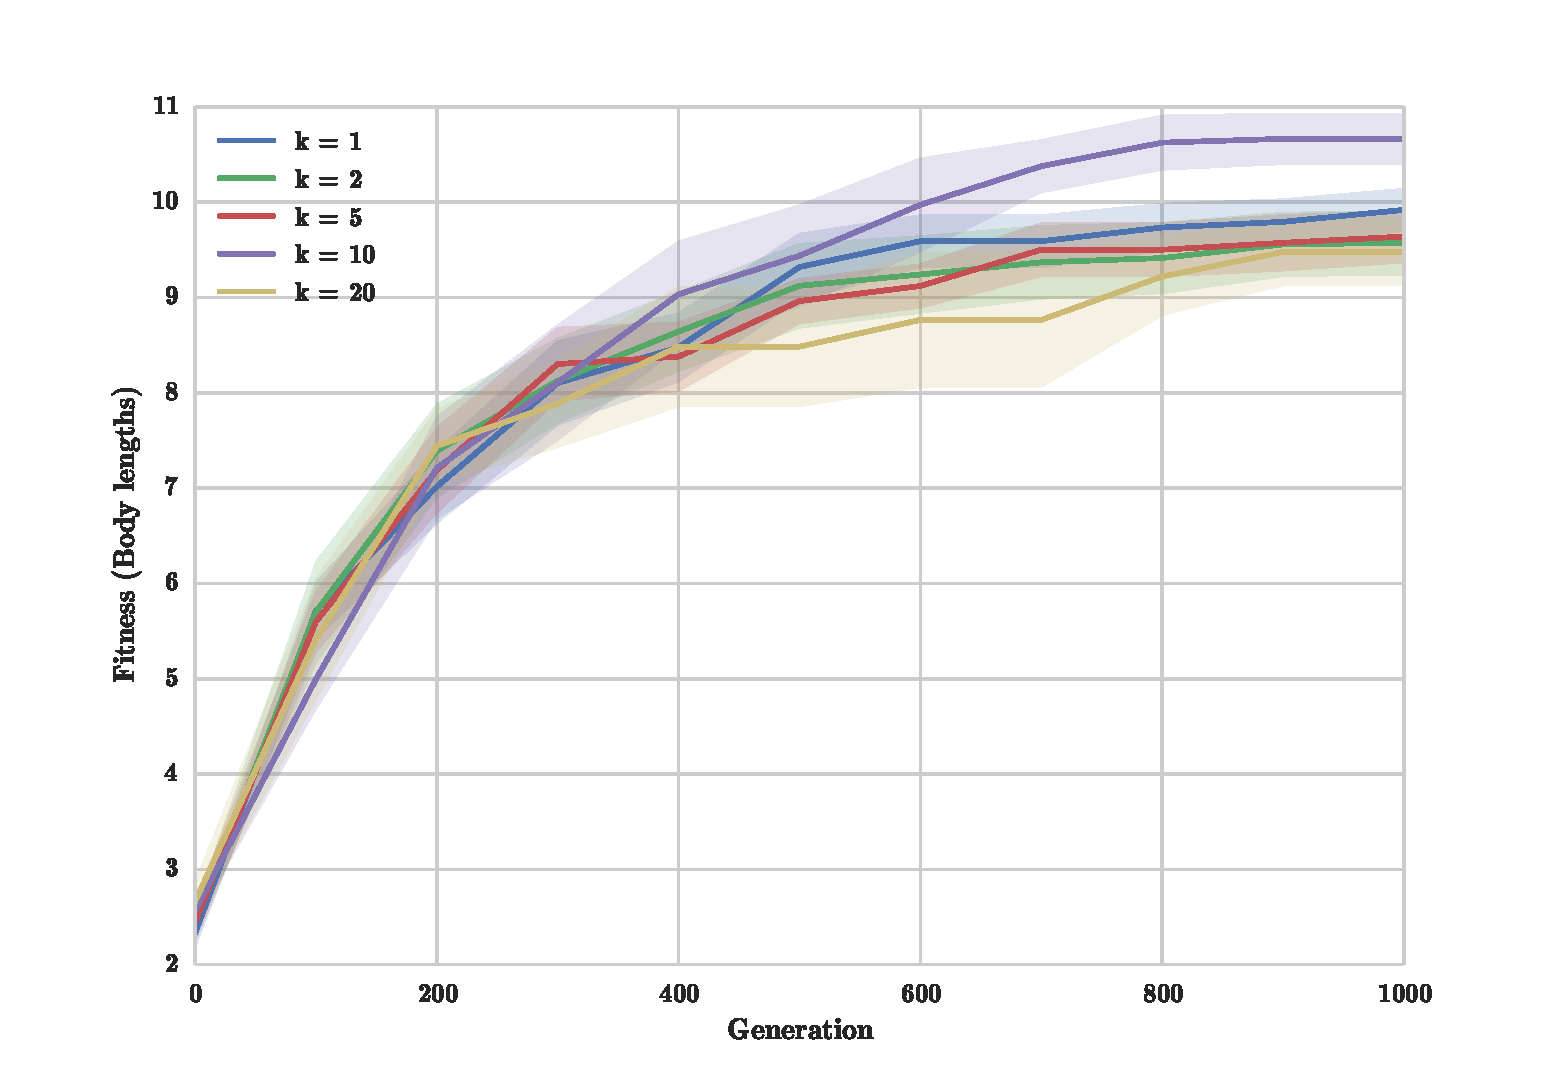
\includegraphics[width=1.0\textwidth]{../Figures/Results/KnnExperimentSize5.pdf}
\caption{Best so far fitness averaged over $10$ runs, for different $k$ to sparsity computation of the behavior. (Settings~\ref{Settings-size5})}
\label{fig:KnnExperimentSize5}
\end{figure}


Sparsity (see Eq.~\ref{sparsenessEquation}) is a metric that evaluates how sparse is the space of a newly generated-observed behavior. In this equation $k$ defines how many of the closest neighboring behaviors are going to be used for the computation of the average distance. Figure~\ref{fig:KnnExperimentSize5} presents the resulted best so far fitness given different values for $k \in \lbrace 1, 2, 5, 10, 20 \rbrace$. In principle $k$ can define how tolerate the algorithm can be with new behaviors. It is not certain that a specific value for $k$ should give the highest performance in fitness and it depends almost completely by the application. The only implication in choosing value for $k$ is that choosing large values should yield in a more detailed exploration in the behavior space, in the contrary using small values the final set of behaviors will be denser in the behavior space. In the specific figure and experiment $k=10$ was the setting that led to the best performance.







